\documentclass{article} 

\usepackage[margin=0.9in]{geometry}
%\usepackage{subfig}
\usepackage{amsmath}
\usepackage{amsfonts}
\usepackage{amssymb}
\usepackage{amsthm}
\usepackage{graphicx}
\usepackage[hidelinks]{hyperref}
% \usepackage{showlabels}
\usepackage{lineno}
% \linenumbers
\usepackage{natbib}

\newtheorem{lemma}{Lemma}
\newtheorem{prop}{Proposition}
\newtheorem{thm}{Theorem}
\newtheorem{prob}{Problem}
\newtheorem{defn}{Definition}
\newtheorem{obs}{Observation}
\newtheorem{alg}{Algorithm}

\newcommand{\median}{\operatorname{median}}

% http://bytesizebio.net/2013/03/11/adding-supplementary-tables-and-figures-in-latex/
\newcommand{\beginsupplement}{%
        \setcounter{table}{0}
        \renewcommand{\thetable}{S\arabic{table}}%
        \setcounter{figure}{0}
        \renewcommand{\thefigure}{S\arabic{figure}}%
     }

\hyphenation{Ge-nome Ge-nomes hyper-mut-ation through-put}

\title{A Literature Review on Quantitative Assays in Viral Immunology}
\author{Jared Galloway | Fred Hutchinson CRC}

\begin{document}
\maketitle

\begin{abstract}
Protection from rapidly spreading and evolving viruses is key to human health and survival.
The molecular nature of infection and respective immune system defences presents us with a complex and noisy set of problems to solve if we are to combat infectious disease and understand the nature of their evolution.
Most notably, we need to understand the affinity of a virus to bind to a host cell via proteins expressed on the surface of the cell's outer membrane.
These proteins allow the virus to enter a host cell, then proceed to hijack the cell's own machinery to replicate and propagate an infection within the host individual.
In the context of SARS-CoV-2, understanding the immune response with respect to those binding proteins is critical for prevention and prediction of disease severity.
Additionally, understanding the evolution of these binding sites allows us to interpret active selection among the viral population
and duration of immunity post-infection using mutational routes of binding escape.
Neither of these are trivial problems to solve.
Fortunately, recent advances in next generation sequencing (NGS), oligonucleotide synthesis (ONS), and PCR-induced mutagenesis have driven the development of quantitative assays and given us the ability to explore and quantify fitness of particular proteins in the context of binding affinity to entry sites on host cells.
These methods have laid the foundation for rapid exploration and development of advanced vaccines providing protection against deadly pathogens.
In this literature review, we explore two techniques which leverage \textit{quantitative assays}; Phage Immunoprecipitation Sequencing (PhIP-Seq) and Deep Mutational Scanning (DMS).
In short, these methods allow us to measure and explore binding properties of relevent proteins and thus, provide insight into the nature of a virus with respect to it's \textit{pathogenisis}.
Concretely, we will provide background and motivation of quantitative assays by observing the results and methods from \citet{Shrock2020} and \citet{Starr2020} -- 
two studies which focus on the binding properties of the novel betacoronavirus, SARS-CoV-2 and it's potential variants.
The primary motivation behind the literature review is to provide and approachable explanation of novel techniques which are being used to rapidly characterize how we are combating novelviral outbreaks.
%Here we're using the SARS-CoV-2 virus as a model but it should be noted these techniques can and have been applied to a much wider variety of ??
% Further we explore the modeling and analysis techniques necessary to parse and query the resulting data from these protocols.
\end{abstract}

\paragraph{Primer \& Prologue}
\textit{You are welcome to skip this section if you're well versed the history and relevance of the Central Dogma and Basic Viral Biology. 
For me, priming myself with the basics before diving deep into complex topics like the ones described in this paper is always beneficial}.

~

Every organism on earth is the aggregate of many underlying biological systems which work together to drive the complex functions which fully characterize every individual.
In more detail, each biological system is driven by a defined set of proteins -- each encoded and regulated by a relatively small portion the individual's genetic code.
Each protein has a role to play which may be trivial by itself, but in concert with the other relevant proteins we observe incredible functionality. 
The advent of Next Generation Sequencing (NGS) and complimentary algorithms has provided researchers with the ability to explore entire genome sequences from almost any living organism of interest.
% Question: is the RNA Genome all protein coding
Even more impressively, we can profile these protein coding portions of the genome by extracting messenger ribonucleic acid (mRNA) from cells to infer the set of all expressed proteins, known as the \textit{proteome}. 
In contrast to living organisms the genetic code of a virus is extremely simplistic. 
In the case of RNA viruses such as SARS-CoV-2, genomes are consisted mostly of protein coding RNA with a severely limited set of instructions.
With no means to replicate or produce energy alone, the singular function of viral proteins is to bind to complimentary proteins expressed on host cells and hijack the machinery in order to reproduce itself - a process which then destroys the cell.
Unfortunately in this specific context (along with many other facets of functional biology), little is known about how the underlying peptide sequences and relates to it's folding properties (tertiary structure) and most importantly, it's primary function.
Exploring the function of proteins and their properties is a necessity when uncovering the labyrinth of biological systems and developing therapeutics to combat disease.

\section*{Introduction}

% Introduce the immune system
Modern mammalian immune systems are constituted by the aggregate of proteins and specialized cells known as \textit{lymphocytes} which
defend against unwanted invaders (pathogens).
These defences keep the pathogens from harming the delicate and complex biological systems which keep us alive and healthy.
However, deadly pathogenic outbreaks which rapidly spread among humans and other species can often harm or kill a large percentage of populations \citep{Wu2020}.
In the case of viruses, replication as a function of fitness drives pathogens to evolve much in the same way we do --
often meaning the most potent and infectious pathogens prevail as a product of their genome evolution \citep{Twiddy2003, Felsenstein1981-zs}.
Fighting fire with fire, the adaptive immune system works through similar processes of mutation and selection, inside our own body,
to evolve along-side these pathogens and confer specialized immunity - in many cases this lasts throughout the lifetime of an individual.
Incredibly, the combinatorial effects of specialized (VDJ) recombination results in enough diversity to select upon that evolution of specialized cells
takes place in mere days (often a week or so) when encountering a new pathogen \citep{Jung2004}.


% Motivate the importance of quantitative assays.
In contrast to all other forms of evolution (often on ecological timescales), 
The process of generating specific antibodies to ward off an infection is incredibly fast.
Unfortunately, the symptoms of an infection during that time frame can still make an individual very ill, or even be fatal.
The ability of viruses to hijack our cell's own machinery to replicate itself in order to propagate the infection make them efficient and deadly.
Luckily, the process of producing antibodies need not occur every time we encounter the same virus.
Rather, once an individual has encountered a pathogen and created the necessary cells needed to fend off the virus and infected cells,
the defences that were used are stored in a sort of ``immuno-memory" -- using another type specialized cell.
Upon contact with a pathogen the individual has encountered in the past, then,
the immune system has the infrastructure in place to elicit a fast and effective response, 
Having this cellular machinery is what's known as immunity in an individual - and is key to survival in a world filled with microbial pathogens.


% context of vaccines
One of the most impactful developments in human health has been our ability to provoke immunity to common
viruses without actually infecting us with a deadly disease causing pathogen.
These biologically prepared agents are known as \textit{vaccines}, 
and according to the center for disease control (CDC.gov) will have prevented over $21,000,000$ hospitalizations and roughly $750,000$
deaths among children born within the last $20$ years -- in the U.S alone.
While this is an extreme success, the rate at which vaccines can be produced are a function of our ability to observe the physical properties of a virus.
To date, the fastest a vaccine has been successfully developed was during the mumps outbreak in 1969 and took 4 years from start to finish.
Facing a more deadly pathogen, of which we are certain exists, this slow rate of development could pose an existential threat to the human race.


% Introduce epitopes, and how phip-seq can be used, briefly
Commonly, a vaccine for some particular virus essentially models the virus - without any of the harmful properties.
This can be thought of as giving your immune system a molecular picture of the virus so that it is prepared when the real thing is encountered.
Anything that elicits an immune response is known as an \textit{antigen} -- the antigen targeted by antibodies for a particular set of pathogens is known as the \textit{epitope}.
Knowing the epitope for any virus is key in modeling it for vaccines.
Inferring a particular antigen is no trivial process, the number of possible peptides chains forming a protein which constitute the epitope for any particular virus are nearly infinitesimal \citep{Stoddard2020}.
To date there is no direct way to isolate which proteins are expressed on a virus, and which constitute an antigen.
% Explain how mutation plays a rold and how deep mutational scanning can be used. 
To complicate further, little is known about how sequence variation affects protein function.
As viruses evolve, we would like to know how possible mutations impact our immuno-defences; 
In the case of the novel coronavirus, SARS-CoV-2, high mutation rates have already been found in the region which binds to our cells.
In order to predict or understand how long immunity will last in the face of evolution, we must explore all variants of the epitope
and their respective binding affinity relative to the wild type sequence.


% explain which advances have been made and make clear what a quatitative assay is
Fortunately, recent advances in techniques such as next generation sequencing (NGS), oligonucleotide synthesis (ONS), modern computing and more, have opened the door to a new brute force, high throughput approach to answering these questions.
% These advances have provided the tools necessary to study pathogen specific proteins and their respective immuno-related (humoral) responses across many individuals.
The conjunction of these  advancements tools have provided the infrastructure necessary to create and analyze \textit{Quantitative assays} in immunology.
Using the related protocols and analysis techniques, researchers now have the ability to explore the relevant likelihoods of nearly every single possible antigen -- as well as every possible mutant of a particular antigen.
These large scale studies require complex and carefully executed protocols resulting in noisy data for analysis \citep{Mohan2018}.
Once the data is acquired complex modeling and computing techniques are applied to parse the signal and produce some form of likelihood surrounding a particular sequence.
This likelihood then informs a great deal about the biological nature of an evolutionary tango between pathogens and the modern immune system.
Quantitative assays in Immunology, particularly in the last decade, have laid the foundation for measuring protein interactions between a virus and individual host cells at magnitude far greater than previously thought possible \citep{Fowler2014, Bloom2014}.


% what are we going to do
Here, we dig into the benefits and limitations of two such quantitative assays, Phage Immunoprecipitation Sequencing (PhIP-Seq), and Deep Mutational Scanning (DMS) along with a hybrid technique, coined Phage-DMS. 
We will explore the methods, results, and analysis tools of two studies applied to proteins expressed by SARS-CoV-2.
These studies will act as a template for understanding the biological insight provided by quantitative assays as a whole.
First, we explore \citet{Shrock2020}, a large-scale PhIP-Seq study done at Harvard university to characterize the set epitopes found in SARS-CoV-2.
Next, we observe how every single mutation across one particular epitope on the novel coronavirus effects the affinity of binding to ACE2 receptor on human cells in \cite{Starr2020}, where the authors used DMS.
Finally, we see how these techniques are combined to offer insight into potential mutational pathways of escape from antibody recognition in \citet{Garrett2020}.
Together, these studies motivate the use quantitative assays and associated analysis techniques in Immunology.

\section*{Quantitative Assays in the Context of SARS-CoV-2}

% should this be part of the intro?
The RNA genome of SARS-CoV-2 consists of $\approx 30,000$ nucleotides which provide the landscape for $11$ protein coding regions \citep{Naqvi2020}.
Of those, there exists a very small subset of less than $90$ nucleotides encoding for a epitopes identifying the virus to lymphocytes and invoking an immune response able to combat the infection.
Designing effective therapeutics and understanding how their effectiveness as the virus evolves over time provokes two primary questions (among many others):
(1) Given the viral genome, how can we accurately infer the correct epitope which will act as the appropriate antigen and 
(2) how effective will the chosen antigenic sequence be in the face of inevitable genome evolution as a result of mutagenesis over time.
In this section we explore two recent studies which leverage commonly used quantitative assay techniques in the field of viral immunology to explore these specific questions. 
For each of these we describe the methods and results, and follow up with future directions and limitations.

\subsection*{Phage Immunoprecipitation Sequencing (PhIP-Seq)}

% TODO Make sure this is the first paper to describe phip
Addressing the question of inferring the profile of virus epitopes targeted by individual antibodies, we turn to one of the more notable quantitative assay techniques, known as Phage Immunoprecipitation Sequencing (PhIP-Seq).
Originally, \citet{Larman2011} introduced a this method which used oligonucleotide synthesis to create a synthetic representation of all possible proteins generated by the human proteome.
This quantitative assay was then used to identify which human proteins were being mislabeled as pathogens, thus leading to auto-immune diseases such as Diabetes type I, multiple sclerosis, and rheumatoid arthritis.
These such libraries are commonly referred to as \textit{peptidomes} \citep{Mohan2018}.
Importantly, the entire span of possible proteins that may be expressed is created using a sliding window approach across the proteome.
The sliding window begins at the start codon and spans some number of codons to encode for all possible proteins that may be expressed given the entire sequence.
The window then jumps some number of codons down the sequence to create an adjacent (and usually overlapping) protein encoding.
This processes continues throughout an open reading frame until all possible protein encoding sub-sequences of oligonucleotides are included in the library.
It should be noted that the chosen size of the tile and how how much overlap each tile shares with adjacent tiles will control the granularity of the assay and thus, the detail of the resulting data.
Once the library is designed, oligonuceotide synthesis is used to generate all genetic information encoding for all proteins of interest in the library.
The oligo encodings are then cloned into a phage vector display (usually T7 phage).
Once cloned, the protein coding nucleotides of interest are then conveniently transcribed using the machinery of the phage and expressed on the exterior to create a peptidome library.


The overarching concept of this technique is to create and label (barcode) a set of proteins of interest - this is the quantitative assay.
Once developed, this assay is then presented (\textit{homogenized}) with serum antibodies extracted from a patient of interest.
Finally, the binding interactions we care about are extracted (precipitated) using specialized magnetic beads to be sequenced.
When the samples are aligned with the library of oligonucleotides, we can count the number of each peptide which had a binding affinity with the antibodies.
The resulting data from this process is then a counts array for which each count represents the number of binding events for each of the peptides in the library.
When repeating this process with multiple samples, the arrays for each are merged to create what is most commonly referred to as the \textit{enrichment matrix}.
It then follows that large numbers in the counts matrix represent some underlying binding affinity of a particular antibody to a specific peptide.
With respect to epitope detection in viruses of interest, this same technique is applied using the proteome of the virus to explore which proteins are targeted by antibodies produced during the infection of some patient or individual.
The first application of PhIP-Seq for viral epitope profiling was presented in \citet{Xu2015}, where the authors developed a peptidome library encapsulating all known human-infecting viruses -- the \textit{Virscan} library.
Virscan contains over 100,000 proteins and offers the most broad view of potential epitopes to date.
Since the introduction of this technique in immunology, a multitude of libraries for viral epitopes have been created and used in subsequent studies to identify detailed maps of individual antibody binding repertoires 
Next, we explore how PhIP-Seq has been used to profile the antibody binding affinities and potential epitopes of SARS-CoV-2.


\paragraph{Peptidomes to profile SARS-CoV-2 epitopes}
In \citet{Shrock2020}, the immune (humoral) response of a mixed cohort of both COVID-19 positive and pre-pandemic individuals ($232$ and $190$, respectively) was quantified by presenting IgG and IgA antibody (\textit{serological}) samples to a set of synthetic peptidomes using PhIP-Seq.
This large scale study provided insight into many outstanding questions surrounding differential immune response to COVID-19.
In addition to the Virscan peptidome described above, the authors present three additional synthetic peptidomes, each to provide a different scope and granularity of candidate epitopes across viral proteomes of interest.
One of the libraries focused specifically on including proteins from all human-infecting coronaviruses (HCoV's).
Among the HCoV's, this included four endemic coronaviruses which cause the common cold including OC43, HKU1, NL63, and 229E and three severe acute respiratory disease causing pathogens SARS-CoV, MERS, and SARS-CoV-2.
The above library encapsulated all protein coding regions from the virus genomes with a 56-mer amino acid (aa) windows tiling every 28aa.
For a more detailed look at SARS-CoV-2 specifically, the authors presented a library across the virus with 20-mer aa windows across the viral proteome tiling every 5aa.
Finally, the authors produce a library across the SARS-CoV-2 proteome with 56-mer aa windows tiling at every codon, except at each location the introduce a triple alanine mutation to precisely define epitope boundaries.
In total across all samples and libraries, this study measured more than $10^{8}$ unique peptide-antibody binding interactions.
Using these individual profiles, the authors explore questions about COVID-19 disease outcome and SARS-CoV-2 epitopes which may be shared with other common human coronaviruses (HCoV's).


\paragraph{SARS-CoV-2 Epitopes and cross-reactivity with endemic HCoV's}
The authors analyze the enrichment matrix looking for significant enrichments among background noise by using a z-score approach and assigning p-values to each of the enrichments.
The subset of significant enrichments among the unique sample-peptide enrichments are suggestive of a biological response when faced with a specific antigen and thus, revealing the profile of epitopes for each sample.
The initial results presented provide evidence SARS-CoV-2 specific epitopes along the Spike (S) and Nucleocapsid (N) proteins of the virus.
In total, the authors identified 823 unique epitopes across the viral proteome.
Severity of COVID-19 disease in an individual has been correlated with a variety of demographics and comorbidities \citep{Yuki2020}.
However, variance of infection outcome within these groups suggests also that individuals viral exposure history plays a role in combating infection.
Shared epitopes across viruses is known as \textit{cross-reactivity}.
To understand which exposures may be cross-reactive with SARS-CoV-2 antibodies, the authors profiled pre-pandemic sample and found significant binding events to SARS-CoV-2 peptides.
This result points out how exposure history plays a large role in infection outcome and may explain the large number of asymptomatic carriers of the disease. 

\paragraph{Predicting SARS-CoV-2 infection history} 
To understand a virus' behavior among a population, rapid testing for past infection is key.
The binding profile of any individual to key proteins involved infection give insight into their viral history and thus, provide an avenue to accurately detect previous infection of the SARS-CoV-2 virus.
The authors presented a machine learning model that used z-score enrichment values as input and predicted the infection status of COVID-19.
The model used the XGBoost algorithm which results in a random forest of decision trees to create a binary classifier.
The binary prediction model was trained on all of samples serum samples using their respective infection status as COVID-19 positive or pre-pandemic as the target.
K-fold cross validation was used to reveal $99\%$ Sensitivity and $98\%$ specificity of the model.
Shap plots were used to reveal the most significant peptides involved with the prediction and found significant overlap with the epitopes specific to SARS-CoV-2.
These results present the amount of information to be gained using binding profiles exposed using the PhIP-Seq technique.

\subsection*{Deep Mutational Scanning (DMS)}

Understanding how underlying amino acid sequences relates to the function (\textit{phenotype}) of proteins remains at large in many facets of biology.
In the case immunology, we are interested in the process by which a pathogen leads to diseased state in an individual - known as \textit{pathogenesis} \citep{Araya2011, Fowler2014, Weile2018}.
We know, for instance, that more than half of human disease is caused by sequence mutations, or single nucleotide polymorphisms (SNPs) \citep{Stenson2009}.
Unfortunately, the lack of ability to map a sequence to the respective phenotype poses a large problem when developing therapeutics or predicting the pathogenic outcome of mutation in a pathogen.
%Unfortunately, it remains unknown how any particular sequence of underlying a protein relates to it's folding properties and overall function.
To address the difficulty, \citep{Araya2011} popularized a method which uses mutagenesis to instead explore how sequence variation changes the binding properties of protein when compared to the wild type protein of interest -- this method is known as Deep Mutational Scanning (DMS).
Taking advantage of the advancement and scaling of next generation sequencing, this method generates a quantitative assay containing every possible amino acid substitution along the protein of interest and then infers how each performs outside of a living organism (in vitro).
Presented in \citet{Adams2016}, the author show how this brute force approach to mutagenesis and subsequent measuring of binding affinity of an antibody to a antigen of interest allow us to explore the function of a protein at the sequence level.

In the context of viruses, each virus infects cells by attaching to a protein on the surface of the host cell via a binding site of it's own.
It then follows that mutations to the binding sites on these viruses would regulate it's affinity to bind, and thus, regulate the infectious properties of the virus.
In \citet{Bloom2014}, the authors explore how the seasonal A/WSN/1933, H1N1 influenza virus is able to escape immunity through mutation.
Using DMS, the authors were able to show how Influenza hemagglutinin -- the flu's integral protein for binding to host cells -- has a high tolerance to mutation in regards to it's binding affinity.
In other words, mutations which may allow the virus to escape recognition and destruction by lymphocytes in the immune system, seem to consistently retain properties which allow for viral entry.
Given this study and other, DMS has been proven itself as a valuable tool to uncover the nature of mutation in relation to their respective modes of host cell viral entry.
Below, we dive into the results from a study exploring the binding affinity of SARS-CoV-2 RBD mutants to the human ACE2 receptor.

\paragraph{Measuring binding affinity of SARS-CoV-2 RBD mutants to human ACE2 receptor}
The entry receptor on host cells for SARS-CoV-2 is the angiotensin converting enzyme 2 (ACE2).
The Receptor Binding Domain (RBD) of the virus' Spike (S) protein encodes for the protein responsible for viral entry as a result to binding to ACE2.
Given this knowledge it would be very relevant to understand how mutations on the RBD impact the mutant's binding affinity to the ACE2 receptor.
Additionally, known variants of SARS-CoV-2 found among infected humans across the globe, mutational impact on the viral binding affinity will also provide evidence about the nature of the selection currently acting on the virus.
In \citet{Starr2020}, the develop a yeast surface-display library of nearly all possible mutations along the Spike protein of SARS-CoV-2 and subsequently measure the change in binding affinity to ACE2.
In other words, the authors performed PCR-induced mutagenesis to produce $3,804$ of the $3,819$ possible RBD amino-acid mutations of the protein coding sequence.
Each variant produced was then linked to a unique $16bp$ barcode using long-read PacBio SMRT sequencing \citep{Matreyek2018}.
Next, the sequences were cloned into a library of yeast which then displayed the full tertiary structure of the respective proteins on the exterior of the fungus.
Using techniques introduced in \citet{Adams2016} and \citet{Peterman2016}, the combination of fluorescent-activated cell sorting (FACS) and deep sequencing was used to measure the ACE2 expression levels, as well as their respective binding affinity to ACE2, for each RBD variant in the libraries. 
By identifying the distribution of read counts among bins of level of RBD expression (measured using fluorescent intensity), Each variant's mean fluorescent intensity (MFI) was identified.
The binding affinities of each variant were presented as the log fold change in compared to the wild type RBD, $\Delta log(MFI)$.
Titration curves as described in \citet{Peterman2016} were fit to each of the variants to infer dissociation constants, $K_{D, app}$ and were reported as $\Delta log_{10}(K_{D, app})$.
In short, this method allowed the authors to measure the binding affinity (fitness) of each nearly each of the possible 19 amino acid substitutions along the SARS-CoV-2 RBD, relative to the wild-type sequence.

\paragraph{Results of RBD variant binding affinity and viral evolution}
The measure of mutant binding affinity reveals many insights into mutational tolerance of the SARS-CoV-2 RBD.
As expected single amino acid substitutions are generally deleterious when compared with the wild type.
This finding would comply with the well-established fact that amino acid substitutions generally impede the folding and general function and folding of most proteins as described in \citet{Soskine2010}.
However, the authors present the result that $46\%$ of single amino-acid mutations along the RBD retain the ability to bind relatively well to ACE2 suggesting high mutational tolerance.
With a large number of targeted epitopes in the RBD, this finding would suggest many potential mutational paths of escape from immunity in individuals while retaining the ability to infect host cells.
In contrast many of the targeted epitopes have more mutational tolerance than those of the RBD in direct contact with ACE2, suggesting clever epitope targeting may limit the potential pathways of escape for SARS-CoV-2.
To explore how existing mutations may be selected for currently, $31,570$ sequences of isolated RBD sequences were observed from human samples and observed 98 mutations.
Of all mutations found, 56 were observed in only a single sample presenting the low frequency of viral mutation and selection.
The binding affinities of the observed mutations from human samples had significantly less deleterious affects when compared to random mutations, suggesting purifying selection among the viral population.
Importantly, nearly all mutations present in human samples had nearly neutral change in binding affinity, which would seem to mean there is no positive selection for more aggressive mutants in the population to date.

\section*{Conclusions and Discussion}

In this literature review, we have explored the benefit of using quantitative assays and their associated protocols to gain insight into key properties of viral infections.
We provide background and difficulty of exploring protein function given underlying amino acid sequence.
We explore studies focused on SARS-CoV-2, the novel betacoronavirus responsible over a million deaths worldwide to date, as a motivating example for the use and advancement of these methods.
We explain the history behind these methods and how each is an aggregate of several historical advancements in a large variety of molecular and computational techniques including but not limited to Next Generation Sequencing, Oligonucleotide Synthesis, and induced mutagenesis across a genetic sequence of interest.
The urgency of combating disease sheds light on urgency of advancing these quantitative assays to measure protein function and fitness in the context of viral immunology.

We summarized PhIP-Seq, a brute force approach to synthesizing the span of all possible proteins of interest across a proteome, and subsequently measures their binding affinity to samples antibodies.
We reviewed \citet{Shrock2020} which explored, in detail, the landscape of SARS-CoV-2 epitopes revealed by antibodies from a large cohort of individual serum antibodies.
This study provided insight into the specific epitopes unique to SARS-CoV-2 as well cross-reactive epitopes with related coronaviruses.
The data generated from this protocol gave enough statistical power to outperform state-of-the-art SARS-CoV-2 infection history testing.
A shortcoming of current PhIP-Seq methods limits us to exploring \textit{linear epitopes}.
What this means is that the proteins expressed on phage 

This review explained the basic methods driving DMS and it benefits when exploring mutational impact on protein functionality.
While we explored this method in the context of viral immunology, it should be noted that this technique has broad implications and potential for exploring genotype to phenotype maps at the level of proteins -- and outstanding and crucial problem in functional biology.
By exploring the key results from \citet{Starr2020}, we described evidence about the current forces of evolution acting on the SARS-CoV-2 virus in humans.
Additionally, the evidence provided suggested that the RBD of SARS-CoV-2 had high tolerance in the face a single mutation in it's ability to retain viral entry function.
Fortunately, the data provided may help design broadly neutralizing antibodies limiting escape, and thus allowing us to confer long-term immunity against the virus.

For brevity, this review avoids the complex analysis and computational techniques necessary for exploring the large resulting datasets.
Instead, we focus on the background, explanation, and relevant results.
Unfortunately, this overlooks an aspect of these protocols which currently acts as a bottleneck in exploring the resulting data.
Indeed, both PhIP-Seq and DMS give us datasets which are relatively large and noisy -- highlighting accurate modeling a necessity in order to avoid false positive results from inherent bias introduced by various steps of each respective protocol.

In conclusion, this literature review hopes to explain and motivate the power of quantitative assays when exploring protein function in viral immunology.
It does not critique many aspects of each method which act as shortcomings in their ability to clearly provide results.
PhIP-Seq provides a platform the gives a profile of antibody binding affinity for each sample which is presented tot he library and subsequently sequenced.
When the samples are combined, patterns can be observed to provide insight into the biological mechanisms of the immune system in response to a given virus.
Researchers can leverage this information to develop the most effective vaccines and therapeutics target the pathogen and prevent it's proliferation in individuals.
DMS has laid the foundation for exploring protein function as a whole simply by observing it's change in function when compared to all possible 19 amino acid substitutions.
The information about protein variants gives us crucial information about the current forces of evolution of a virus in real time during a pandemic such as the spread of COVID-19.


%\begin{figure}[h]
%\centering
%\includegraphics[width=0.35\textwidth]{figures/subsplit.pdf}
%\caption{\
%A subsplit structure.
%}%
%\label{fig:}
%\end{figure}

% \begin{figure}[h]
% \centering
% \includegraphics[width=0.35\textwidth]{figures/subsplit.pdf}
% \caption{\
% A subsplit structure.
% }%
% \label{fig:subsplit}
% \end{figure}


% \bibliographystyle{plain}
% \bibliography{main}

\bibliographystyle{plainnat}
\bibliography{main}

\section*{Supplementary Figures}

\begin{figure}[h]
\centering
\includegraphics[width=0.75\textwidth]{figures/PhIP-Seq-Cartoon.jpg}
\caption{lsjfln}
\label{fig:PhIP-Seq-Cartoon}
\end{figure}

\begin{figure}[h]
\centering
\includegraphics[width=0.35\textwidth]{figures/DMS-Cartoon.jpg}
\caption{lsjfln}
\label{fig:DMS-Cartoon}
\end{figure}

\begin{figure}[h]
\centering
\includegraphics[width=0.65\textwidth]{figures/Starr-Methods.jpg}
\caption{lsjfln}
\label{fig:Starr-Methods}
\end{figure}


\begin{figure}
\centering
\begin{tabular}{cc}
  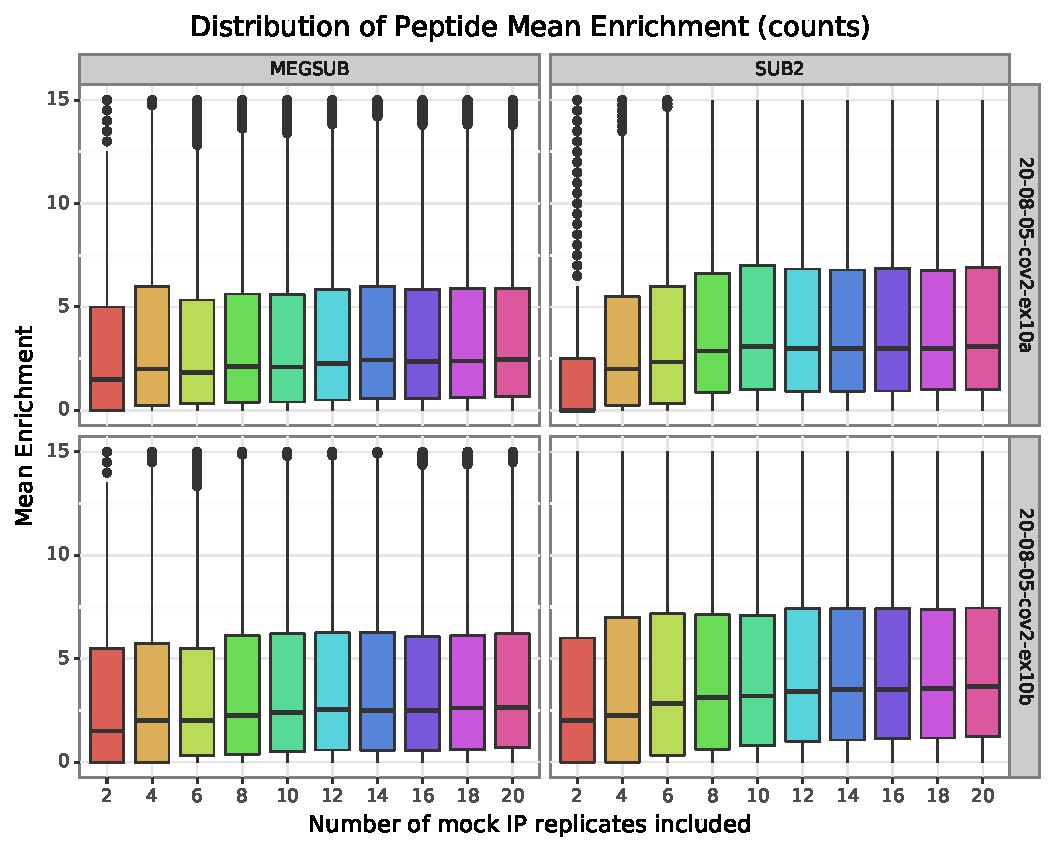
\includegraphics[width=65mm]{figures/42_mockip_abundance_variance/counts/mean_limit_y.pdf} &   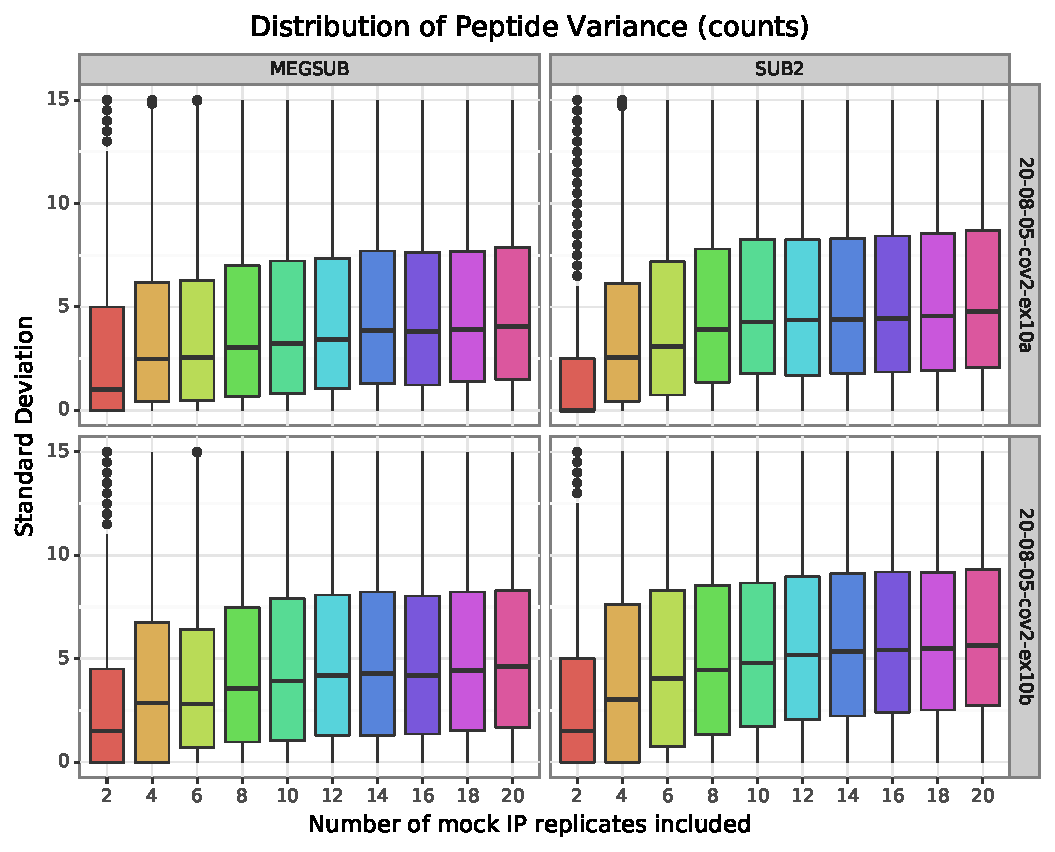
\includegraphics[width=65mm]{figures/42_mockip_abundance_variance/counts/std_limit_y.pdf} \\
(a) first & (b) second \\[6pt]
% 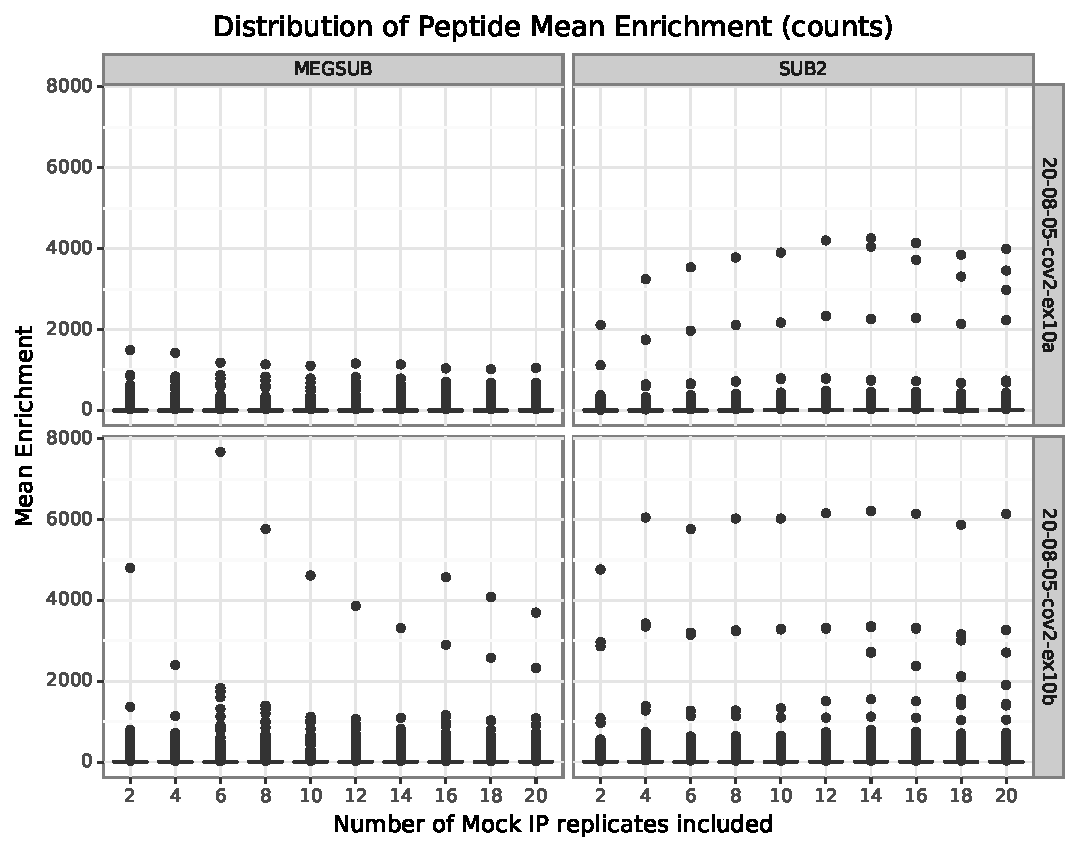
\includegraphics[width=85mm]{figures/42_mockip_abundance_variance/counts/mean.pdf} &   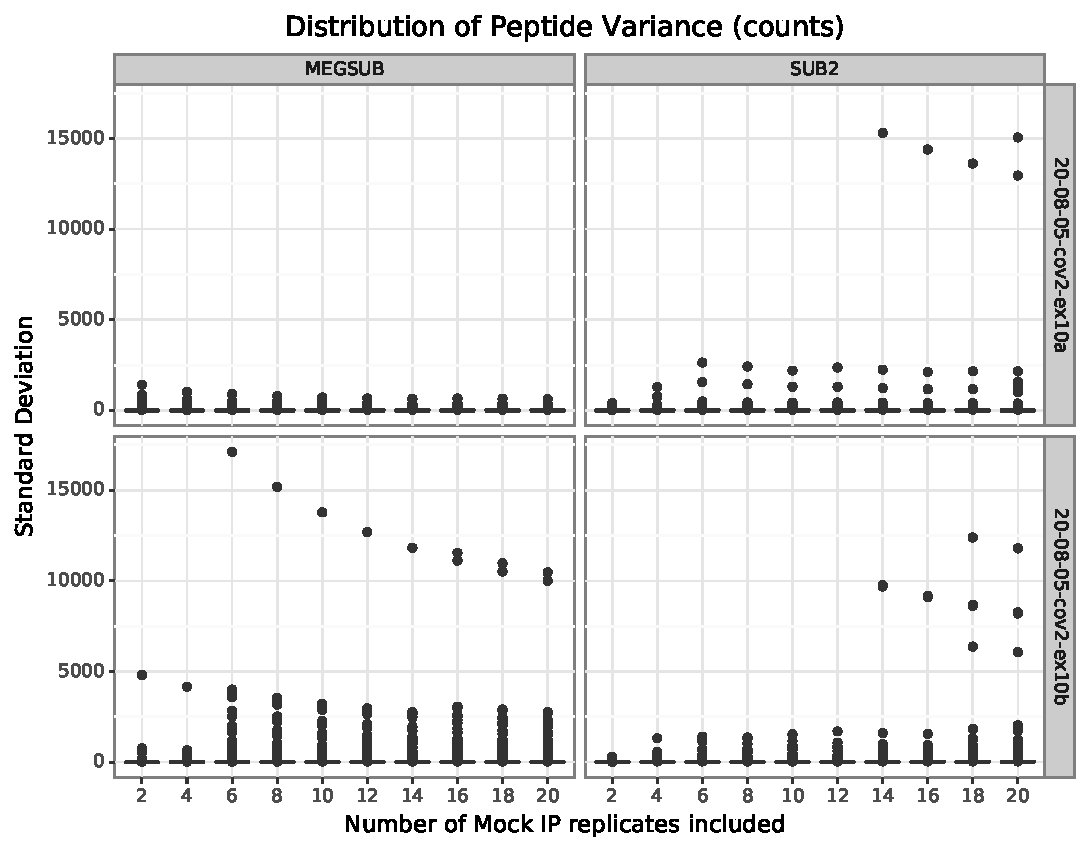
\includegraphics[width=85mm]{figures/42_mockip_abundance_variance/counts/std.pdf} \\
%(c) third & (d) fourth \\[6pt]
\multicolumn{2}{c}{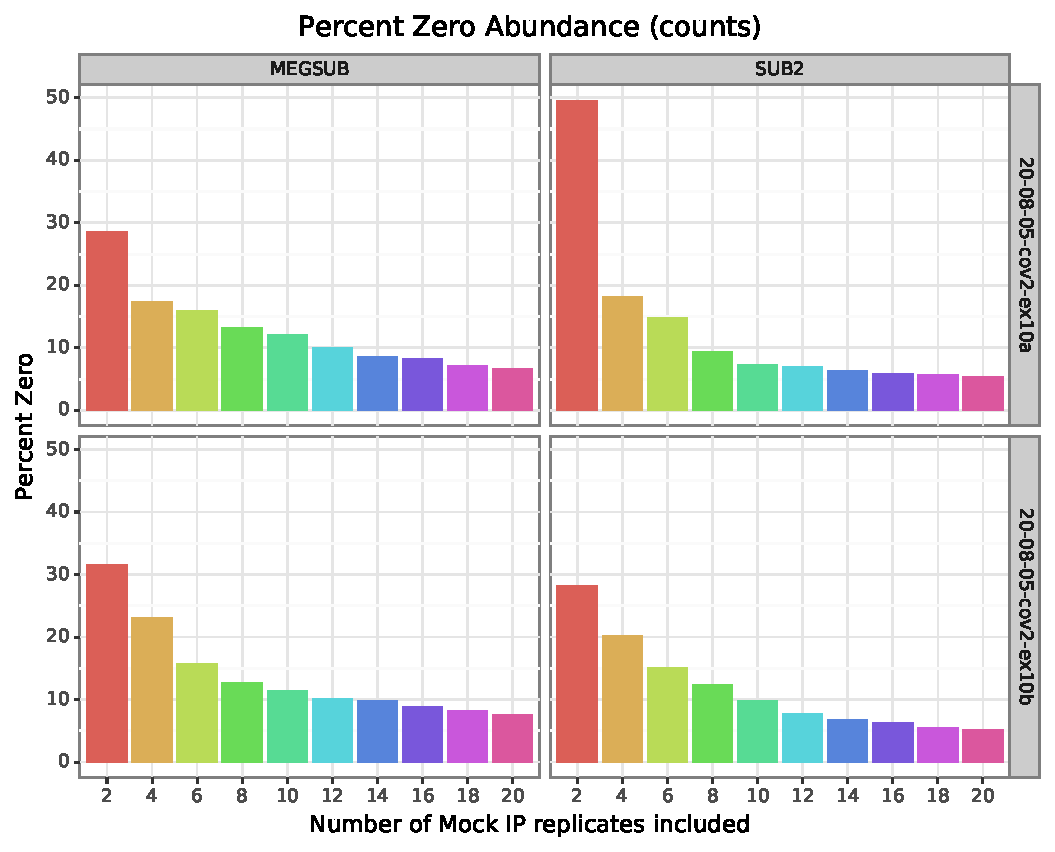
\includegraphics[width=85mm]{figures/42_mockip_abundance_variance/counts/per-zero.pdf} }\\
\multicolumn{2}{c}{(e) fifth}
\end{tabular}
\caption{caption}
\end{figure}

% \clearpage
% \section*{Supplementary Materials}
% \beginsupplement
% Supplementary text and figures here.


\end{document}
